\usepackage[utf8]{inputenc}
\usepackage[T1]{fontenc}
\usepackage{mathptmx}
\usepackage[scaled=.90]{helvet}
\usepackage{courier}
\usepackage{caption}
\captionsetup{labelformat=empty,labelsep=none}
\usepackage{verbatim}
\usepackage{hyperref}
\usepackage{listings}
% strikethrough (\sout)
\usepackage{ulem}
\lstset{language=Perl,basicstyle=\normalsize,tabsize=3,showstringspaces=false}

\title{Dancer and DBIx::Class}
\author[racke]{Stefan Hornburg (Racke)\\ \texttt{racke@linuxia.de}}
\date{Czech Perl Workshop, Prague, 21st May 2014}

\begin{document}
\maketitle{}

\begin{frame}
  \titlepage
\end{frame}

\tableofcontents

% \section{Übersicht}

% DBIx::Class ist mit Sicherheit einer der größten Schätze von "Modern Perl"
% und bietet schnelle und komfortable Datenbankabfragen.

% Ebenso erleichtert Dancer das Erstellen von Webanwendungen mit einer leicht
% verständlichen Programmierung.

% Wie können beide zusammen genutzt werden? Zunächst mit dem DBIC Plugin für
% Dancer. Mit diesem können mehrere DBIx::Class Schemas innerhalb der
% Dancer-Anwendung verwenden werden.

% Um auch die Dancer-Sessions in der Datenbank zu speichern, habe ich eine Engine für Dancer und DBIC geschrieben.

% Außerdem werde ich ein Projekt vorstellen, mit dem man einfach den Inhalt
% von Datenbanken mittels eines DBIx::Class Schemas editieren kann.

% \begin{frame}<handout:0>{Übersicht}
% \begin{itemize}
% \item Einführung
% \item DBIC Schemas mit Dancer Plugin
% \item DBIC session engine
% \item TableEditor
% \end{itemize}
% \end{frame}

% Wir starten mit einer kurzen Einführung von DBIx::Class.

\section{Introduction}
% \begin{frame}{Datenbank}
% \begin{itemize}
% \item Datenbank
% \item Tabellen
% \item Datensätze
% \end{itemize}
% \end{frame}

% \begin{frame}{DBIx::Class}
% \begin{itemize}
% \item Schema
% \item ResultSet
% \item Row / Objekt
% \end{itemize}
% \end{frame}

\subsection{Dancer}

Let's dance. I'm Racke from Hannover.pm in Germany and work
as self employeed programmer and system administrator.

My presentation is about Dancer and DBIX::Class and how to use
them in conjunction.

I started to develop Dancer applications 3 years ago
after listening to an amazing presentation from sawyer
at FOSDEM in Brussels.

There are a couple of reasons that made Dancer my favourite web
framework.
 
\begin{frame}{Easy to start with}
\begin{itemize}
\item Application ready to go
\item Syntax easy to understand
\item Routes and Keywords
\end{itemize}
\end{frame}

\begin{frame}{Easy to expand}
\begin{itemize}
\item Plugins
\item Hooks
\item Engines
\end{itemize}
\end{frame}

\begin{frame}{Solid}
\begin{itemize}
\item Stable
\item Keep behaviour
\item Community
\end{itemize}
\end{frame}

\begin{frame}{Applications}
\begin{itemize}
\item Simple Dropbox 
\url{https://metacpan.org/pod/Dancer::Plugin::Dropbox}
\item .state.gov Websites \\
\url{https://eshop.state.gov/}
\item Monitor for Power Plant
\end{itemize}
\end{frame}

\subsection{DBIx::Class}
\begin{frame}{DBIx::Class}
\begin{itemize}
\item ORM
\item Objects instead of SQL
\item Performance
\end{itemize}
\end{frame}

It took some time to get involved with DBIx::Class for various reasons.

\begin{frame}{DBIx::Class}
\begin{itemize}
\item Table => Result classes
\item users => Interchange6::Schema::Result::User
\item Searches => Result sets
\end{itemize}
\end{frame}

\begin{frame}{User and Roles}
\begin{description}
\item[User]
\begin{itemize}
\item racke@linuxia.de
\item info@nite.si
\item test@linuxia.at
\end{itemize}
\item[Role]
\begin{itemize}
\item user
\item editor
\item admin
\item guest
\end{itemize}
\end{description}
\end{frame}

\begin{frame}{Tables}
\begin{itemize}
\item users
\begin{itemize}
\item users\_id
\item email
\item first\_name
\item ...
\end{itemize}
\item roles
\begin{itemize}
\item roles\_id
\item name
\item label
\end{itemize}
\item user\_roles
\begin{itemize}
\item users\_id
\item roles\_id
\end{itemize}
\end{itemize}
\end{frame}

\begin{frame}[fragile]{Roles for an user}
\begin{lstlisting}
mysql> select R.name from users U
       join user_roles UR on (U.users_id = UR.users_id)
       join roles R on (UR.roles_id = R.roles_id)
       where U.email = 'racke@linuxia.de';

+--------+
| name   |
+--------+
| user   |
| editor |
+--------+
\end{lstlisting}
\end{frame}

\begin{frame}[fragile]{User with DBIx::Class}
\begin{lstlisting}
$rs = $schema->resultset('User');
$user = $rs->find(1);
$user = $rs->find({email => 'racke@linuxia.de'});

$first_name = $user->first_name;

$users_linuxia = $rs->search({
    email => {like => '%@linuxia.de'}});
\end{lstlisting}
\end{frame}

\begin{frame}[fragile]{Roles with DBIx::Class}
\begin{lstlisting}
$rs = $schema->resultset('User');
$user = $rs->find({email => 'racke@linuxia.de'});

$roles = $user->roles;
\end{lstlisting}
\end{frame}

\begin{frame}[fragile]{User Result Class}
\begin{lstlisting}
package Interchange6::Schema::Result::User;

__PACKAGE__->table("users");

__PACKAGE__->add_columns(...);

__PACKAGE__->set_primary_key("users_id");

\end{lstlisting}
\end{frame}


\begin{frame}[fragile]{User Result Class}
\begin{lstlisting}
package Interchange6::Schema::Result::User;

__PACKAGE__->has_many("UserRole",
  "Interchange6::Schema::Result::UserRole",
  { "foreign.users_id" => "self.users_id" },
);

__PACKAGE__->many_to_many("roles", "UserRole", "Role");
\end{lstlisting}
\end{frame}

\subsubsection{Tips and Tricks}

\begin{frame}[fragile]{Object inflation}
\begin{lstlisting}
debug "Role: ", $role;

debug "Role: ", {$role->get_inflated_columns};
\end{lstlisting}
\begin{lstlisting}
Role: {'label' => 'User',
       'name' => 'user',
       'roles_id' => '3'} 
\end{lstlisting}
\end{frame}

\begin{frame}{Object vs Hashref}
\begin{itemize}
\item Debug / Logs
\item Templates
\item API / JSON
\item Speed
\end{itemize}
\end{frame}


\subsection{Database Administration}
\begin{frame}{Database Administration}
\begin{itemize}
\item \sout{phpmyadmin}
\item \sout{phppgadmin}
\item TableEditor
\end{itemize}
\end{frame}

\begin{frame}{TableEditor Features}
\begin{itemize}
\item Different database systems \\
      MySQL, PostgreSQL, ...
\item higher level of abstraction
\item modern frontend
\item concise source code
\item ``simple'' installation
\end{itemize}
\end{frame}

\begin{frame}[plain]{Input Database Parameters}
  \begin{center}
    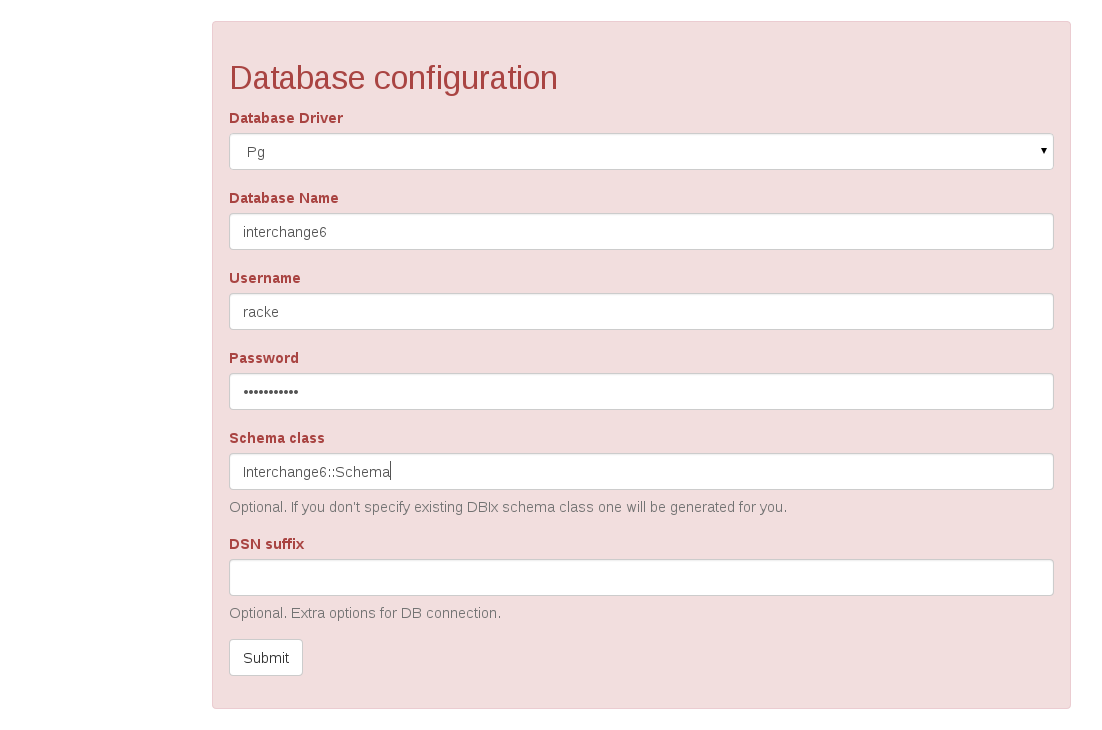
\includegraphics[width=\textwidth,height=1\textheight,keepaspectratio]{images/input.png}
  \end{center}
\end{frame}

\begin{frame}[plain]{View Products}
  \begin{center}
    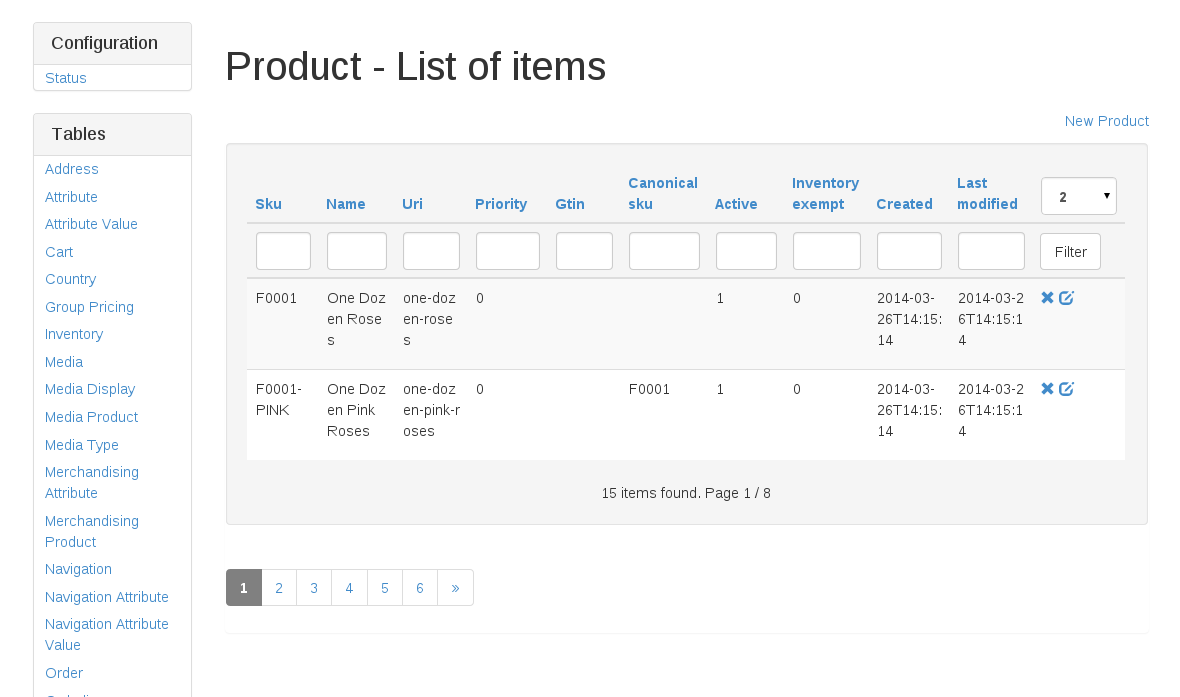
\includegraphics[width=\textwidth,height=1\textheight,keepaspectratio]{images/product.png}
  \end{center}
\end{frame}

\begin{frame}[plain]{View Product}
  \begin{center}
    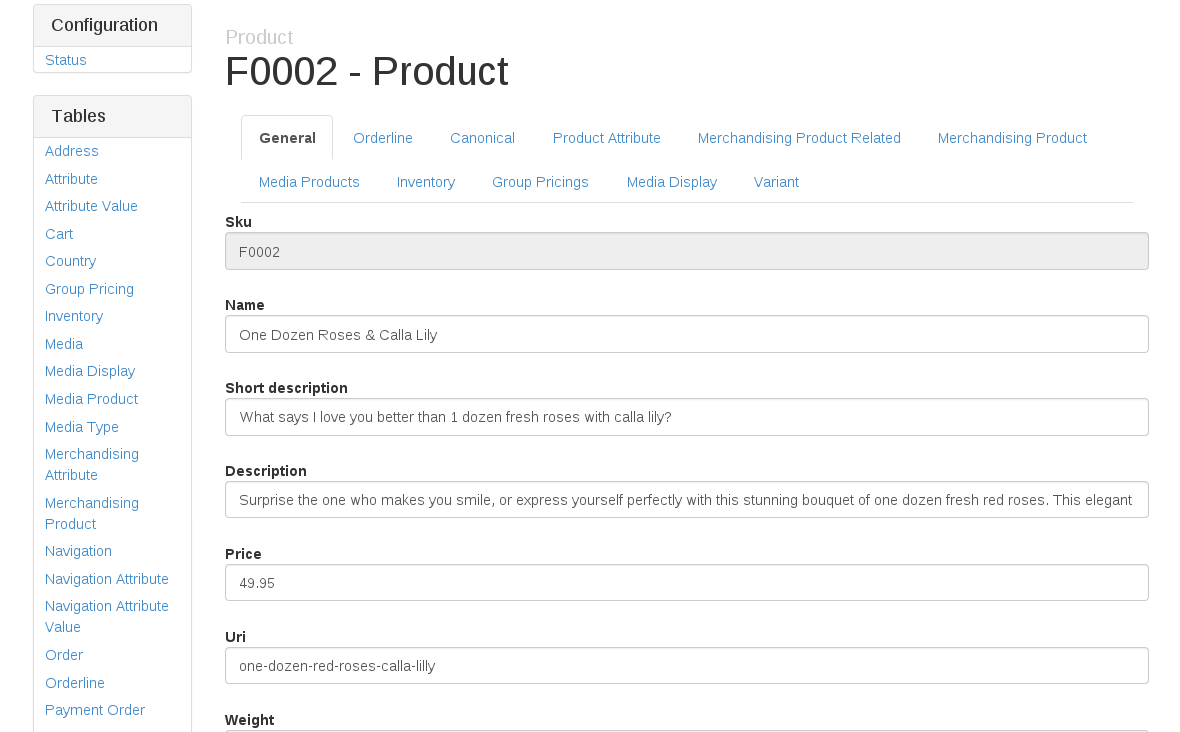
\includegraphics[width=\textwidth,height=1\textheight,keepaspectratio]{images/product-detail.png}
  \end{center}
\end{frame}

\begin{frame}[plain]{Relationship Orderline}
  \begin{center}
    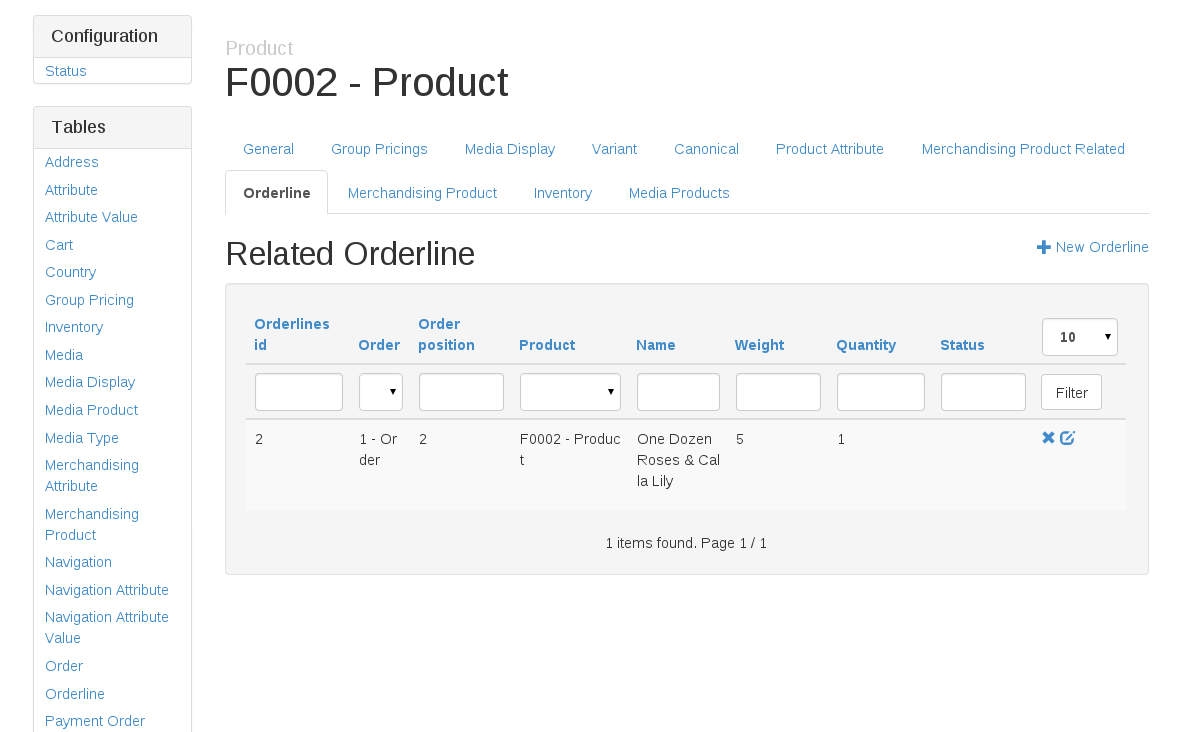
\includegraphics[width=\textwidth,height=1\textheight,keepaspectratio]{images/product-related.png}
  \end{center}
\end{frame}

\section{Dancer::Plugin::DBIC}

\begin{frame}{Overview Dancer::Plugin::DBIC}
\begin{itemize}
\item Usage
\item Configuration
\item UTF-8
\item Create schema dynamically
\end{itemize}
\end{frame}

\subsection{Usage}
\begin{frame}[fragile]{DBIx::Class without Dancer Plugin}
\begin{lstlisting}
use Interchange6::Schema;

$schema = Interchange6::Schema->connect(...);

$schema->resultset('User')->search({..});
\end{lstlisting}
\end{frame}

\begin{frame}[fragile]{DBIx::Class with Dancer Plugin}
\begin{lstlisting}
use Dancer::Plugin::DBIC;

schema->resultset('User')->search({..});

resultset('User')->search({..});

rset('User')->search({..});
\end{lstlisting}
\end{frame}

\subsection{Configuration}

Im Normalfall verwendet man nur ein Schema in seiner
Dancer-Anwendung:

\begin{frame}[fragile]{Configuration}
\begin{lstlisting}
plugins:
  DBIC:
    default:
      dsn: dbi:mysql:interchange6
      user: racke
      pass: nevairbe
      schema_class: Interchange6::Schema
\end{lstlisting}
\end{frame}

Es sind aber auch mehrere möglich:

\begin{frame}[fragile]{Multiple Schemas}
\begin{lstlisting}
plugins:
  DBIC:
    default:
      dsn: dbi:mysql:interchange6
      user: racke
      pass: nevairbe
      schema_class: Interchange6::Schema
    legacy:
      dsn: dbi:mysql:interchange5
      user: racke
      pass: nevairbe
      schema_class: Interchange5::Schema
\end{lstlisting}
\end{frame}

Das Schema \verb|legacy| wird dann wie folgt verwendet:

\begin{frame}[fragile]{Multiple Schemas}
\begin{lstlisting}
use Dancer::Plugin::DBIC;

schema('legacy')->resultset('UserDb')->search({..});
\end{lstlisting}
\end{frame}

\subsection{UTF-8}
Im Gegensatz zu Dancer::Plugin::Database bietet das DBIC-Plugin
keine automatische Unterstützung für UTF-8. Also ist die entsprechende
DBI-Option in der Konfiguration einzutragen, hier für MySQL:
\begin{frame}[fragile]{UTF-8 for MySQL}
\begin{lstlisting}
plugins:
  DBIC:
    default:
      dsn: dbi:mysql:interchange6
      user: racke
      pass: nevairbe
      schema_class: Interchange6::Schema
      options:
        mysql_enable_utf8: 1
\end{lstlisting}
\end{frame}

Die Optionen für die gängigen Datenbanken in der Übersicht:

\begin{description}
\item[SQLite] \verb|sqlite_unicode: 1|
\item[MySQL] \verb|mysql_enable_utf8: 1|
\item[PostgreSQL] \verb|pg_enable_utf8: 1| 
\end{description}

\subsection{Create schema dynamically}
Das DBIC-Plugin erzeugt dynamisch ein DBIx::Class::Schema, wenn
die Schema-Klasse (\verb|schema_class|) nicht angegeben wird.
Dazu ist das Modul DBIx::Class::Schema::Loader erforderlich.

Dies ist nicht empfehlenswert für den Produktionseinsatz, jedoch
praktisch für den TableEditor.

\begin{frame}[fragile]{Create schema dynamically}
\begin{itemize}
\item \verb|schema_class| missing in configuration
\item DBIx::Class::Schema::Loader
\item test and development
\item TableEditor
\end{itemize}
\end{frame}

\section{Dancer::Session::DBIC}

\begin{frame}<handout:0>{Overview Dancer::Session::DBIC}
\begin{itemize}
\item engines
\item configuration
\item serialization
\item session expiration
\end{itemize}
\end{frame}

\subsection{Engines}
\begin{frame}{Engines}
\begin{itemize}
\item Templates \\
TT, Xslate, Flute, ...
\item Sessions \\ 
Storable, Database, DBIC
\item Logger \\
File, Syslog
\item Serializer  \\
JSON, YAML, XML
\end{itemize}
\end{frame}

Die Sessionengines werden in Dancer für gewöhnlich transparent
für den Anwendungscode in der Konfiguration eingerichtet:

\begin{frame}{Configuration}
\begin{description}
\item[session] name of session engine (DBIC)
\item[session\_options] options
\item[session\_expires] expiration date
\end{description}
\end{frame}

Das ermöglicht es, auf dem Liveserver eine effizientere Engine
zu verwenden (z.B. Storable) und auf dem Entwicklungsserver
eine Engine, die einem beim debuggen hilft (z.B. YAML).

Die Optionen für Dancer::Session::DBIC ähneln der Konfiguration von
Dancer::Plugin::DBIC, zusätzlich können wir festlegen wie
die Sessions aus der Datenbank abgerufen werden können:

\begin{description}
\item[resultset] DBIx::Class resultset
\item[id\_column] primary key
\item[data\_column] field for session data 
\end{description}

Das sieht dann z.B. für \href{https://metacpan.org/pod/Interchange6::Schema}{Interchange6::Schema} (Version 0.015) so aus:

\begin{frame}[fragile]{Configuration}
\begin{lstlisting}
session: "DBIC"
session_options:
  dsn: dbi:mysql:interchange6
  user: racke
  pass: nevairbe
  schema_class: Interchange6::Schema
  resultset: Session
  id_column: sessions_id
  data_column: session_data
session_expires: 12 hours
\end{lstlisting}
\end{frame}

Die Konfiguration kann aber ebenso im Hauptmodul
stattfinden:

\begin{frame}[fragile]{Configuration}
\begin{lstlisting}
set session => 'DBIC';
set session_options => {schema => schema};
\end{lstlisting}
\end{frame}

\subsection{Example table}

Folgendermaßen sieht die Tabelle \verb|sessions| aus,
die vom Schema \href{https://metacpan.org/pod/Interchange6::Schema}{Interchange6::Schema} (Version 0.015)
erzeugt wird:

\begin{frame}[fragile]{Example table}
\begin{lstlisting}
CREATE TABLE `sessions` (
  `sessions_id` varchar(255) NOT NULL,
  `session_data` text NOT NULL,
  `created` datetime NOT NULL,
  `last_modified` datetime NOT NULL,
  PRIMARY KEY (`sessions_id`)
) ENGINE=InnoDB;
\end{lstlisting}
\end{frame}

\subsection{Serializer}
\begin{frame}[fragile]{Serializer}
\begin{lstlisting}
set 'session_options' => {
    schema       => schema,
    serializer   => sub { YAML::Dump(@_); },
    deserializer => sub { YAML::Load(@_); },
};
\end{lstlisting}
\end{frame}

\subsection{Session expiration}

Beim Überschreiten der erlaubten Ablaufzeit wird die Sitzung
ungültig, sie wird jedoch nicht in der Datenbank gelöscht.
Dafür ist ein Skript zur regelmäßigen Löschung der
abgelaufenen Datensätze erforderlich.

JSON
andere DBIC connection?
tests?

\begin{frame}[fragile]{Session expiration}
\begin{itemize}
\item remove old sessions from database
\item \verb|Interchange6::Schema::Resultset::Session|
\end{itemize}
\begin{lstlisting}
$schema->resultset('Session')->expire('12 hours');
\end{lstlisting}
\end{frame}

\section{TableEditor}

\begin{frame}<handout:0>{Overview TableEditor}
\begin{itemize}
\item Installation
\item Frontend
\item Routes
\item Login
\item Relationships
% \item Limitations
\item Configuration
\end{itemize}
\end{frame}

\subsection{Installation}
Im günstigsten Fall kann die Installation mit 4 Schritten
erledigt werden:

\begin{frame}[fragile]{Installation}
\begin{lstlisting}
git clone https://github.com/interchange/TableEditor
cd TableEditor
cpanm .
./bin/app.pl
\end{lstlisting}
\end{frame}

\begin{frame}[fragile]{Driver}
\begin{itemize}
\item DBD::mysql
\item DBD::Pg
\item ...
\end{itemize}
\end{frame}

\subsection{Frontend}
Das Frontend für den TableEditor ist mit Angular und Bootstrap erstellt.
Das Theme kann sehr einfach durch Austausch der CSS-Datei für Bootstrap
geändert werden.

\begin{frame}<handout:0>{Frontend}
\begin{itemize}
\item Angular
\begin{itemize}
\item Routes for the frontend
\item XHR requests to REST API
\item JSON
\end{itemize}
\item Bootstrap
\item Theme
\end{itemize}
\end{frame}

\subsection{Routes}
\begin{frame}[fragile]{Routes}
\begin{lstlisting}
get '/:class/:id' => require_login sub {
    # retrieve database record and add relationships
    ...

    return to_json($data, {allow_unknown => 1});
};
\end{lstlisting}
\end{frame}

\subsection{Login}

Für die Integration von Authentifizierung in eine Dancer-Anwendung empfehlen
wir wärmestens das
\href{https://metacpan.org/pod/Dancer::Plugin::Auth::Extensible}{Auth::Extensible}
Plugin.

\begin{frame}{Login}
\begin{itemize}
\item Dancer::Plugin::Auth::Extensible
\item Provider
\begin{itemize}
\item Unix
\item DBIC
\end{itemize}
\item Database \textit{(planned)}
\end{itemize}
\end{frame}

\subsection{Relationships}

Beziehungen werden automatisch angezeigt.

\begin{frame}{Relationships}
\begin{itemize}
\item belongs\_to
\item has\_many
\item might\_have
\item has\_one
\item many\_to\_many \\
      needs to be configured
\end{itemize}
\end{frame}

Filter

Es fehlen Felder in related orderline (Übersicht)

Different DBIC keys

Paging

% \subsection{Limitations}
% \begin{frame}{Limitations}
% \begin{itemize}
% \item Primary key for \textbf{one} column only
% \item Speed (complex schemas)
% \item Error handling
% \end{itemize}
% \end{frame}

\subsection{Configuration}
\begin{frame}[fragile]{Configuration}
\begin{itemize}
\item Auth::Extensible
\item DBIC
\begin{itemize}
\item \verb|default|
\end{itemize}
\end{itemize}
\end{frame}

\begin{frame}{Planned Features}
\begin{itemize}
\item Search (Solr)
\item Select schema
\item Debian packages
\end{itemize}
\end{frame}


\section{Forecast and Contribution}

\subsection{Development}

Das Git-Repository für den TableEditor befindet sich auf Github:

\begin{frame}{Development}
\url{https://github.com/interchange/TableEditor}
\end{frame}

\subsection{Dancer2}

Was ist mit Dancer2 ?

Für Dancer2 existiert bereits ein Plugin:

\url{https://metacpan.org/pod/Dancer2::Plugin::DBIC}

Die Sessionengine und der TableEditor wurden noch nicht auf Dancer2 portiert.

\begin{frame}{Dancer2}
  \begin{description}
  \item[Plugin::DBIC] \url{https://metacpan.org/pod/Dancer2::Plugin::DBIC}
  \item[Session::DBIC] \url{https://metacpan.org/pod/Dancer2::Session::DBIC}
    ported 24th April
  \item[TableEditor] not yet ported
  \end{description}
\end{frame}

% \section{Testing}
% DBIC, Plugin
% Testdatabase

\subsection{Further reading}

\url{https://github.com/castaway/dbix-class-book}

\subsection{Slides}

\begin{frame}{Slides}
Slides:
\url{http://www.linuxia.de/talks/czpw2014/dancer-dbic-en-beamer.pdf}
\end{frame}

\end{document}

%%% Local Variables: 
%%% mode: latex
%%% TeX-master: t
%%% End: 
